\section{Аналитический раздел}

\subsection{Определение параллельного корпуса}

Под <<лингвистическим корпусом>> понимают достаточно объемное собрание примеров языкового массива, определенным образом структурированное, унифицированное и размеченное, объединенное общим логическим замыслом (доминантой), хранящееся в электронной форме, позволяющее решать лингвистические задачи. 
Понятие <<корпуса текстов>> близко к понятию лингвистического корпуса и представляет собой более частную форму проявления последнего. 
В случае корпуса текстов, его доминантой является одна или совокупность определенных целей: обучение иностранному языку, отладка систем машинного перевода и прочие~\cite{maltseva-opredelenie-korpusa-2011}.

Корпус, содержащий тексты только на одном языке, называется монолингвистическим (англ. <<monolingual corpus>>). 
В случае хранения текстов на двух языках, корпус называют билингвистическим (англ. <<bilingual corpus>>).

Параллельный корпус -- билингвистический корпус, содержащий тексты одновременно как на его изначальном языке, так и на некотором другом языке~\cite{khosla-survey-report-2018}.

\subsection{Применение параллельного корпуса}

Параллельный корпус является ценным ресурсом для исследователей самых разных сфер, таких как машинный перевод, перевод с помощью компьютера, изучение языков с помощью электронных ресурсов, переводоведение, контрастивная лингвистика~\cite{spyns-theory-and-applications-NLP-2013}.
Рассмотрим подробнее основные области применения параллельного корпуса: машинный перевод, инструменты обработки естественного языка, языкознание и работа переводчика или преподавателя.

\subsubsection{Машинный перевод}
	
Параллельный корпус является важнейшей частью работы статистических систем машинного перевода, а также систем, работа которых основана на правилах. 
Данные системы постоянно анализируют доступные тексты для вычисления наиболее вероятного перевода. 
Кроме того, параллельный корпус используется и в методе машинного перевода с использованием глубокого обучения.
	
\subsubsection{Инструменты обработки естественного языка}
	
Некоторые инструменты NLP (аббр. Natural Language Processing -- обработка естественного языка) также зависят от параллельного корпуса. 
Примерами таких инструментов являются программы для кросс-языкового извлечения данных (англ. <<Cross Language Information Retrieval>>), транслитерации (побуквенной передачи отдельных слов и текстов одной графической системы средствами другой системы), систем ответов на вопросы (англ. <<Question Answering Systems>>), предназначенных для ответов на вопросы на естественном языке, и другие.
	
\subsubsection{Языкознание}
	
Одно слово в языке может иметь множество значений в зависимости от контекста \cite{poibeau-MT-2017}. 
Таким образом, параллельный корпус помогает в исследованиях влияния окружения слова на его перевод (при наличии достаточного количества загруженных текстов). 
С помощью корпуса выявляются характерные для языка паттерны использования конкретных слов, фраз. 
Кроме того, на основе текстов делаются выводы об особенностях морфологии, синтаксиса языков, а также вытекающих из них особенностях перевода. 
Самым ярким примером науки, которой необходим параллельный корпус, является контрастивная лингвистика.
	
\subsubsection{Работа переводчика или преподавателя}
	
В связи с множеством возможных переводов слова или фразы в зависимости от контекста, работа переводчика неразрывно связана с использованием лингвистических инструментов. 
Как правило, 50\% времени, затрачиваемого на перевод -- это использование справочных материалов~\cite{rura-tranlator-aid-2008}. 
Использование параллельного корпуса призвано облегчить работу переводчика, поскольку корпус содержит множество примеров перевода слов, фраз и предложений в зависимости от контекста их употребления. 
Кроме того, корпус может помочь людям, изучающим иностранный язык.

\subsection{Требования к корпусу}

При создании лингвистического корпуса рекомендуется придерживаться следующих правил \cite{szudarski-corpus-linguistics-for-vocab-2017}.

\begin{enumerate}
	\item Тексты корпуса должны выбираться без учёта специфики языков, на котором они написаны.
	
	\item Содержание корпуса должно быть репрезентативным.
	
	\item Только те компоненты корпуса, которые спроектированны быть независимо контрастивными, должны быть контрастивными.
	
	\item Вся информация о тексте должна храниться отдельно, но может быть объединена при необходимости.
	
	\item Экземпляры текстов, включаемые в корпус, должны добавляться туда целиком (или настолько в целостном состоянии, насколько это возможно).
	
	\item Состав и структура корпуса должны быть задокументированы (иначе корпус бесполезен).
	
	\item Разработчик должен стремиться к созданию разнообразного, сбалансированного корпуса. 
	
	\item Тексты должны быть однородными (гомогенными), следует избегать текстов плохого качества.
\end{enumerate}

Важно отметить, что эти рекомендации важны не столько в терминах практических советов, сколько как указание на важность учета теории при разработке корпуса.

Многие авторы отмечают, что не существует <<идеального>> корпуса. Как указал М. Нельсон, каждая попытка создать корпус суть компромис между ожидаемым и достигаемым \cite{nelson-building-written-corpus-2010}. 
Тем не менее, при попытке создать собственный корпус важно учитывать вышеперечисленные рекомендации.

Что касается размера корпуса, важно учитывать его предназначение. 
Если параллельный корпус требуется для исследования редкоупотребляемых слов, то требуется корпус большого размера, т.е. имеющий большое количество текстов разных авторов из разных жанров. 
В случае обыкновенного перевода или исследования базовых слов языка, такое разнообразие не требуется. 
Таким образом, размер корпуса -- открытый вопрос, который решается для каждого корпуса в отдельности.

Репрезентативность корпуса означает, что корпус учитывает лингвистическое разнообразие данного языка и выбранной темы для исследования. 
Смежное качество -- сбалансированность в отношении структуры корпуса и данных для его заполнения. 
Утверждается, что хорошо сбалансированный корпус содержит несколько подразделов, представляющих разные варианты использования языка (наличие текстов разных жанров). 
Причем важно, чтобы разделы имели примерно одинаковое число слов~\cite{szudarski-corpus-linguistics-for-vocab-2017}.

\subsection{Работа с корпусом}

Рассмотрим этапы работы с корпусом~\cite{spyns-theory-and-applications-NLP-2013}:

\begin{enumerate}
	\item сбор материала для корпуса;
	
	\item выравнивание;
	
	\item разметка;
	
	\item использование корпуса.
\end{enumerate}

Источником данных могут выступать политические документы, инструкции и документации к ПО, переведённые веб-сайты. 
Примерами таких источников можно назвать сайт Европарламента, сайты дипломатеческих представительств или открытую информацию с сайта gnu.org.

Главная задача выравнивания -- способствование поиску переводов. 
В то время как в монолингвистическом корпусе поиск производится с целью извлечения примеров перевода, в параллельном корпусе результатом поиска должны быть и переводы соответствующих примеров употребления. 
В результате выравнивания имеется некоторое соответствие между предложениями (в худшем случае, абзацами и главами) на двух языках.

Разметка добавляет дополнительную информацию в корпус, которая и является преимуществом корпуса над классическими словарями или сборниками текстов. Выделяют несколько видов разметки. Выбор вида разметки зависит от целей исследований, для которых используется корпус.

Выровненный, размеченный корпус является готовым инструментом для исследований. 
Он может служить помощником как переводчику или преподавателю, так и исследователю-лингвисту. 
Основной операцией в корпусе является поиск с указанными параметрами. 
Причем допустимые параметры могут варьироваться от корпуса к корпусу.

\subsection{Разметка параллельного корпуса}

Именно разметка отличает параллельный корпус от обычного собрания текстов. 
Зачастую разметку также называют аннотацией. Выделяются следующие основные виды (уровни) разметки~\cite{annotation-russian}\cite{leech-annotation-schemes-1993}:

\begin{itemize}[label=---]
	\item просодическая;
	
	\item морфологическая (морфосинтаксическая);
	
	\item синтаксическая (грамматическая);
	
	\item семантическая;
	
	\item прагматическая;
	
	\item разметка дискурса;
	
	\item анафорическая (местоименная);
	
	\item метаразметка (параметры текстов).
\end{itemize}

Наличие конкретного вида разметки во многом определяет назначение корпуса. 
Если необходим анализ употребления конкретных грамматических \\форм, требуется грамматическая разметка.

Кроме того, разметка может помочь в поиске точных примеров использования конкретного слова. 
Если, например, необходимо получить все примеры употребления напитков (или предметов одежды) в текстах, необходима семантическая разметка.

Просодическая разметка используется для фиксации ударений в словах и интонации в случае их произношения. 
Она применяется, как правило, в корпусах устной разговорной речи и сопровождается дискурсной разметкой, которая указывает на наличие пауз, повторов или оговорок. Данные виды разметки сложны для автоматизации и проводятся вручную.

Анафорическая разметка фиксирует референтные связи (например, местоименные). Однако, поскольку большая часть программ анализирует тексты, предварительно разбив их на предложения, и, следовательно, связи между предложениями теряются, анафорическая разметка проводится вручную.

Прагматическая разметка применяется для указания прагматических фун-кций фразы, предложения или абзаца. 
Прагматическая функция лингвистической единицы зависит от дискурса, личности повествователя и др., и показывает, как связаны повествователь, его фразы и действия, которые он совершает. 
Автоматизация прагматической разметки также затруднена~\cite{archer-pragmatic-annotation-2008}.

Аннотация текста может быть произведена несколькими способами. 
Во-первых, она может быть проведена полностью вручную. 
Во-вторых, возможен вариант ручной разметки с помощью электронных средств. 
Наконец, существует полностью автоматический вариант разметки. 
Примером разметки, которая может быть проведена полностью автоматически, является морфологическая разметка~\cite{szudarski-corpus-linguistics-for-vocab-2017}.

\subsubsection{Морфологическая разметка}

Определение морфологических форм и значений является самостоятельной научной проблемой. 
Морфологическая информация, приписываемая произвольному слову в тексте, может состоять из следующих полей \cite{annotation-russian}:

\begin{itemize}[label=---]
	\item лексема, которой принадлежит словоформа -- указывается часть речи;
	
	\item множество грамматических признаков лексемы, словоклассифицирующие характеристики (род для существительного, переходность для глагола и т.д.);
	
	\item множество грамматических признаков словоформы, или словоизменительные характеристики (падеж для существительного, число для глагола);
	
	\item информация о нестандартности грамматической формы.
\end{itemize}

Например, в Национальном корпусе русского языка (НКРЯ) \cite{ruscorpora} используется следующая морфологическая разметка на основе латинских букв \cite{annotation-russian}.

\begin{enumerate}
	\item Части речи:
	
	\begin{itemize}[label=---]
		\item \textit{S} -- существительное,
		
		\item \textit{A} -- прилагательное,
		
		\item \textit{NUM} -- числительное,
		
		\item \textit{V} -- глагол,
		
		\item \textit{ADV} -- наречие,
		
		\item \textit{PARENTH} -- вводное слово.\\
	\end{itemize}
	
	\item Значения грамматических категорий \footnote{
	Стоит отметить, что есть языки, в которых отсутствует понятие рода. 
	Пример -- турецкий язык. 
	Нет разницы между <<братом>> и <<сестрой>> -- это все <<kardeş>>. 
	Таким образом, не все перечисленные морфологические признаки могут быть выявлены для слов конкретной языковой пары.}:
	
	\begin{itemize}[label=---]
		\item \textit{m} -- мужской род,
		
		\item \textit{f} -- женский род,
		
		\item \textit{m-f} -- <<общий>> род,
		
		\item \textit{n} -- средний род.
	\end{itemize}

	\item Одушевленность:
	
	\begin{itemize}[label=---]
		\item \textit{anim} -- одушевленный,
		
		\item \textit{inan} -- неодушевленный.
	\end{itemize}

\end{enumerate}

\subsubsection{Метаразметка}

Под метаразметкой понимается приписывание тексту атрибутов, отражающих обстоятельства его создания, автора, тематику, жанровые особенности и другие. 
Цель метаразметки -- разграничить тексты разного качества, разных жанров, разной даты написания для получения наиболее релевантных ответов относительно запроса \cite{annotation-russian}.

Частые атрибуты для указания параметров текста:

\begin{itemize}[label=---]
	\item автор текста,

	\item время создания текста,

	\item объем текста,

	\item название текста,

	\item жанр (тип) текста,

	\item тематика текста.
\end{itemize}

В случае подхода к наполнению корпуса с помощью интернета (т. н. Web Mining Approach), логично также указывать ссылку на источник, режим, время и дату доступа \cite{khosla-survey-report-2018}.

\subsubsection{Синтаксическая разметка}

В случае синтаксической разметки, каждому предложению текста приписывается его синтаксическая структура. 
Существует множество моделей синтаксической структуры предложения. 
Например, НКРЯ использует лингвистическую модель И.А. Мельчука <<Смысл $\mathrel{\Leftrightarrow}$ текст>>. 
В данной модели синтаксическая структура представляет собой дерево зависимостей, в узлах которого стоят слова предложения, а дуги помечены именами синтаксических отношений \cite{annotation-russian}.

Пример синтаксического дерева для предложения <<Виктор сдал экзамен>> представлен на рисунке \ref{syn-tree}.

\begin{figure}[ht]
	\centering
	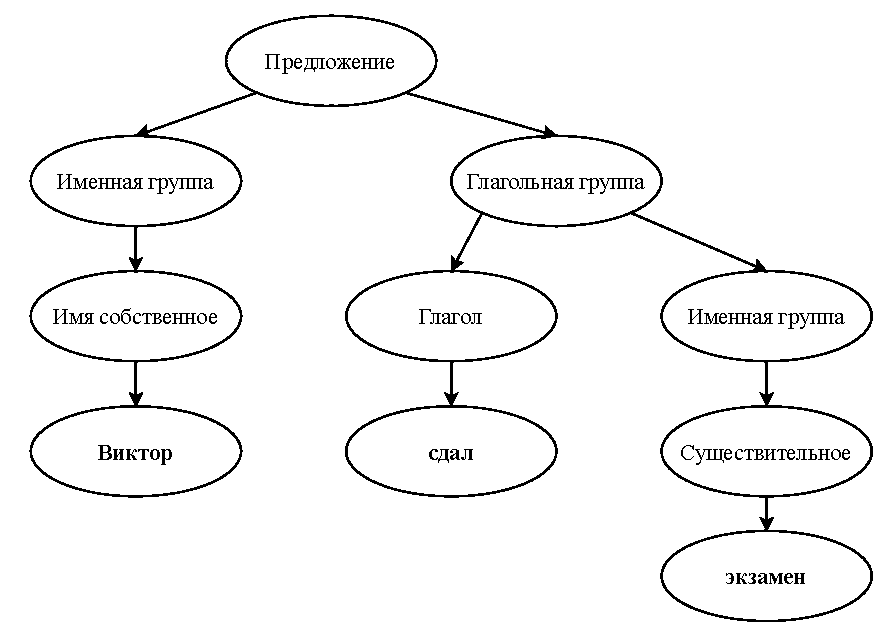
\includegraphics[width=\textwidth]{img/syn-tree.pdf}
	\caption{Пример синтаксического дерева}
	\label{syn-tree}
\end{figure}

Синтаксическая разметка -- сложная задача, которая для каждого языка решается индивидуально.
Более того, синтаксическая разметка плохо применима в средствах машинного перевода \cite{poibeau-MT-2017}. 
Её использование оправдано при проведении специальных исследований. 

\subsubsection{Семантическая разметка}

При данной разметке большинству слов в тексте приписываются один или несколько семантических или словообразовательных признаков. 
Примерами признаков могут быть движение, вещество, одежда, свойство человека и т.д. 
При этом одно слово может попадать в несколько классов.

Семантическая разметка -- крайне трудная задача из-за проблемы многозначности слов. 
Трудно отнести слово, которое имеет десятки значений при разном контексте, к конкретному выделенному классу \cite{annotation-russian}.

\subsection{Требования к базе данных и хранимой информации}

В соответствии с описанной спецификой хранения данных в параллельном корпусе текстов, разработанная база данных должна соответствовать следующим требованиям.

\begin{itemize}[label=---]
	\item В базу данных загружаются тексты в текстовом формате с минимальной, заранее описанной аннотацией (метаразметкой текста).
	
	\item После загрузки текста должно быть произведено выравнивание текста по предложениям, затем предложений по словам.
	
	\item После выравнивания по словам, должна быть произведена морфологическая аннотация каждого слова.
	
	\item Должна быть возможность быстрого поиска по базе данных для получения перевода слова, примеров употребления слова в предложениях с возможностью указать параметры разметки: морфологические признаки слова или изменить параметры выборки текстов.
	
	\item Система должна быть расширяема до любого количества языков.
	
	\item Должна быть предоставлена возможность совместного использования корпуса.
\end{itemize}

Поскольку семантическая и синтаксическая аннотация сложны и используются чаще всего только при специализированных исследованиях, их наличие от корпуса не требуется. 
К морфологической и метаразметке предъявляются следующие требования:

\begin{itemize}[label=---]
	\item по каждому слову (кроме его перевода) текстов должна быть информация о его исходном языке, части речи, грамматической категории и одушевленности;
	
	\item о каждом тексте должна быть известна информация о его авторе, времени доступа к информации, объему текста (в предложениях), названии и его жанре. 
	В случае онлайн источника, должна быть указана ссылка на источник.
\end{itemize}


\subsection{Существующие решения}

Как отмечается, не существует универсальной архитектуры для построения корпуса \cite{khosla-survey-report-2018}. 
Большинство существующих решений используют XML (eX-tensible Markup Language) \cite{xml}, HTML (HyperText Markup Language) \cite{html} и TXT файлы для хранения корпуса. 
В редких случаях используют Excel файлы~\cite{khosla-survey-report-2018}. 
В последнее время стали появляться корпусы на основе реляционных баз данных~\cite{tao-ruschi-corpus-2015}~\cite{pezik-polish-2011}.

При этом стоит отметить, что самое распространенное решение -- XML файлы -- обладает рядом недостатков \cite{pavlov-xml-to-sql-2004}.

\begin{itemize}[label=---]
	\item Синтаксис XML избыточен;
	
	\item Долговременное хранение XML-документа нерационально: его размер существенно больше бинарного представления тех же данных;
	
	\item Избыточность XML может повлиять на эффективность приложения.
	Возрастает стоимость хранения, обработки и передачи данных;
	
	\item Cкорость поиска по корпусу будет равна скорости поиска по текстову документу, заполненного, кроме основного текста, большим числом тегов разметки.
\end{itemize}

Однако XML данные подходят для загрузки данных в базу для их дальнейшей обработки вне этого файла. \pagebreak

Пример организации загрузки XML файла представлен на рисунке \ref{xml-to-sql} \cite{pavlov-xml-to-sql-2004}.

\begin{figure}[ht]
	\centering
	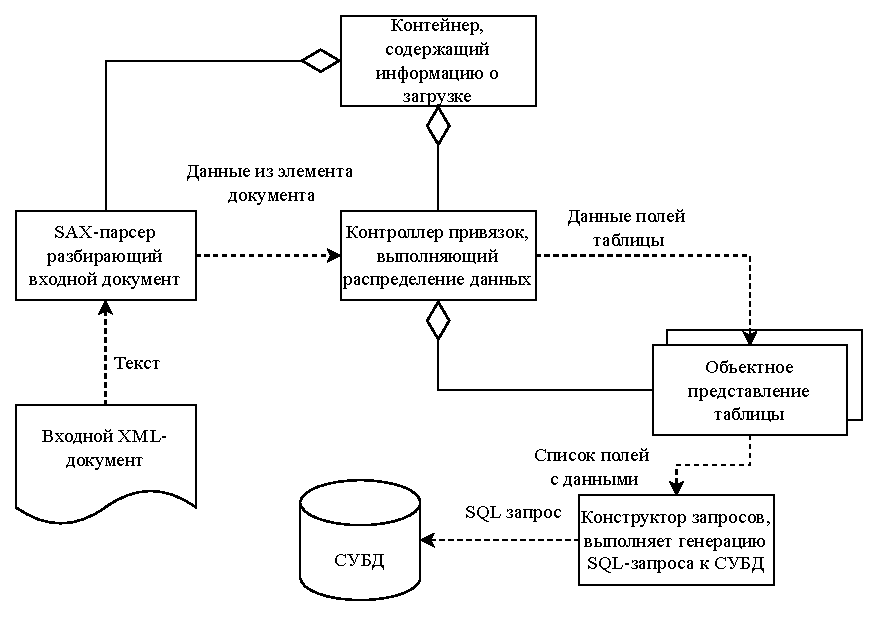
\includegraphics[width=\textwidth]{img/XmlToSql.pdf}
	\caption{Пример организации загрузки XML документов в СУБД}
	\label{xml-to-sql}
\end{figure}

Что касается примеров существующих решений, выделяются следующие продукты: Reverso~\cite{reverso}, Abbyy Lingvo~\cite{abbyy-lingvo} и Linguee~\cite{linguee}. 
Преимущества и недостатки этих продуктов представлены в таблице~\ref{comparison}.

\begin{table}[H]
	\caption{Сравнение существующих решений}\label{comparison}
	\begin{tabular}{|l|l|l|}
		\hline
		Продукт &
		Преимущества &
		Недостатки \\ \hline
		Reverso &
		\begin{tabular}[c]{@{}l@{}}--- поддержка;\\ --- большая база текстов.\end{tabular} &
		\begin{tabular}[c]{@{}l@{}}--- платная подписка;\\ --- нельзя фильтровать тексты;\\ --- нельзя загружать тексты.\end{tabular} \\ \hline
		Abbyy Lingvo &
		\begin{tabular}[c]{@{}l@{}}--- возможность добавления \\      собственных материалов.\end{tabular} &
		\begin{tabular}[c]{@{}l@{}}---прекращена поддержка;\\ --- ориентированность на \\      словари вместо текстов;\\ --- нельзя фильтровать тексты.\end{tabular} \\ \hline
		Linguee &
		\begin{tabular}[c]{@{}l@{}}--- поддержка;\\ --- большая база текстов;\\ --- наличие как словаря, \\ так и  переводчика.\end{tabular} &
		--- нельзя фильтровать тексты. \\ \hline
	\end{tabular}
\end{table}

Из приведенного анализа видно, что общий недостаток существующих решений -- отсутствие возможности самостоятельной загрузки текстов или хотя бы поиска по определенной выборке текстов. 
Также недостатком является необходимость платной подписки для получения полного функционала в некоторых решениях.

\subsection{Анализ существующих СУБД}

Рассмотрим существующие системы управления базами данных, но сначала определим основные понятия.

База данных (БД) – это самодокументированное собрание интегрированных записей \cite{krenke-db-design-2005}.

\begin{enumerate}
	\item БД является самодокументированной, т.е. она содержит описание собственной структуры. 
	Это описание называется словарем данных, каталогом данных или метаданными.
	
	\item БД – это собрание интегрированных записей, она содержит:
	
	\begin{itemize}[label=---]
		\item файлы данных,
		
		\item метаданные,
		
		\item индексы,
		
		\item метаданные приложений.
	\end{itemize}

	\item БД является информационной моделью пользовательской модели предметной области.
\end{enumerate}

Выделяют следующие требования к архитектуре базы данных \cite{guschin-db-2015}.

\begin{itemize}[label=---]
	\item Каждый пользователь должен иметь возможность обращаться к одним и тем же данным, используя свое собственное представление о них. 
	Каждый пользователь должен иметь возможность изменить свое представление о данных, причем это изменение не должно оказывать влияния на других пользователей.
	
	\item Пользователи не должны непосредственно иметь дело с подробностями физического хранения данных в базе.
	
	\item Администратор базы данных должен иметь возможность изменять структуру хранения данных в базе, не оказывая влияния на пользовательские представления.
	
	\item Внутренняя структура базы данных не должна зависеть от таких изменений физических аспектов хранения информации, как переход на новое устройство хранения.
	
	\item Администратор базы данных должен иметь возможность изменять концептуальную или глобальную структуру базы данных без какого-либо влияния на всех пользователей.
\end{itemize}

Система управления базами данных (СУБД) -- это совокупность программ и языковых средств, предназначенных для управления данными в базе данных, ведения базы данных и обеспечения взаимодействия её с прикладными программами. При этом СУБД должна обеспечивать совместное использование данных многими пользователями, безопасность данных, эффективный интерфейс доступа к данным \cite{karpova-db-textbook-2009}.

Классификация СУБД проводится по нескольким признакам. 
Рассмотрим классификацию по модели данных и по архитектуре организации хранения данных~\cite{karpova-db-textbook-2009}~\cite{guschin-db-2015}.

\subsubsection{Модели данных}
Выделяют следующие СУБД по используемой ими модели данных~\cite{guschin-db-2015}.
\begin{itemize}[label=---]
	\item Дореляционные:
	
	\begin{itemize}[label=---]
		\item инвертированные списки (файлы),
		
		\item иерархические,
		
		\item сетевые.
	\end{itemize}
	
	\item Реляционные.
	
	\item Постреляционные.
\end{itemize}

Иерархическая модель может быть представлена как древовидный граф с записями в виде узлов и множествами в виде ребер.
Схема иерархической архитектуры представлена на рисунке~\ref{ierarch}.
\pagebreak

\begin{figure}[ht!]
	\centering
	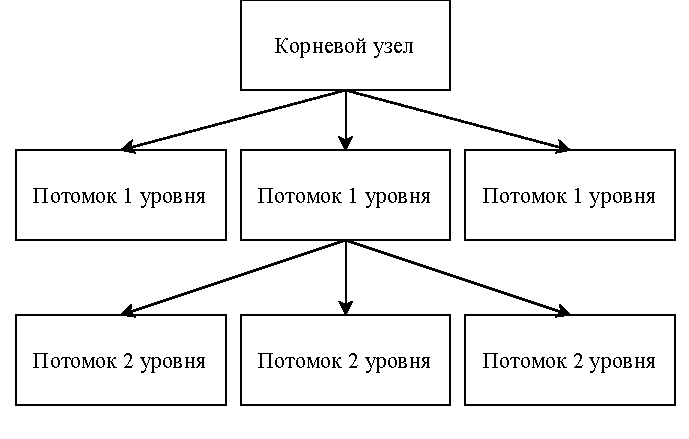
\includegraphics[scale=1]{img/ierarch.pdf}
	\caption{Схема иерархической архитектуры}
	\label{ierarch}
\end{figure}

В иерархической модели узел может иметь только одного родителя. 
Узлы представляют собой интересующие нас объекты, а связи между ними определяются указателями, содержащими в себе информацию о физическом расположении данных~\cite{guschin-db-2015}. 
Структура узла представлена на рисунке~\ref{ierarch-struct}.

\begin{figure}[ht]
	\centering
	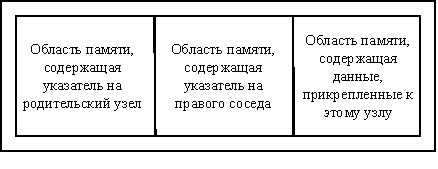
\includegraphics[scale=1.5]{img/ierarch-struct.pdf}
	\caption{Структура узла}
	\label{ierarch-struct}
\end{figure}

Сетевой подход является развитием иерархической архитектуры: потомок может иметь любое число предков. 
В сетевой модели логика процедуры выборки данных зависит от физической организации этих данных. 
Таким образом, модель не является полностью независимой от приложения: 
если необходимо изменить структуру данных, то придется модифицировать и приложение~\cite{guschin-db-2015}. Пример сетевой модели представлен на рисунке~\ref{netw}.\pagebreak

\begin{figure}[ht]
	\centering
	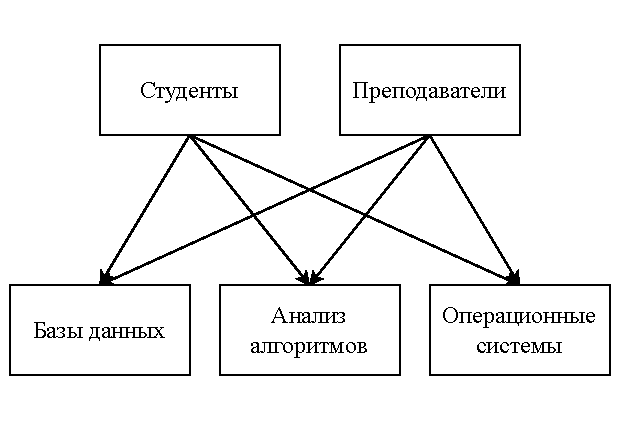
\includegraphics[scale=1]{img/netw.pdf}
	\caption{Пример сетевой модели данных}
	\label{netw}
\end{figure}

СУБД на основе инвертированных списков представляет собой совокупность инвертированных файлов, отличающихся простотой организации и наличием весьма удобных языков манипулирования данными \cite{guschin-db-2015}.
База данных на инвертированных списках состоит из таблиц отношений, однако она сильно отличается от реляционной модели. 
В такой модели данных отсутствуют ограничения целостности, допускается сложная структура атрибутов. 
Все ограничения на возможные экземпляры БД задаются теми программами, которые работают с БД. 
Пользователь может управлять логическим порядком строк в каждой таблице с помощью специального инструмента -- индексов. 
Эти индексы автоматически поддерживаются системой и явно видны пользователям \cite{avrunev-db-models-2018}. Пример организации инвертированных списков представлен на рисунке~\ref{invert}.

\begin{figure}[ht]
	\centering
	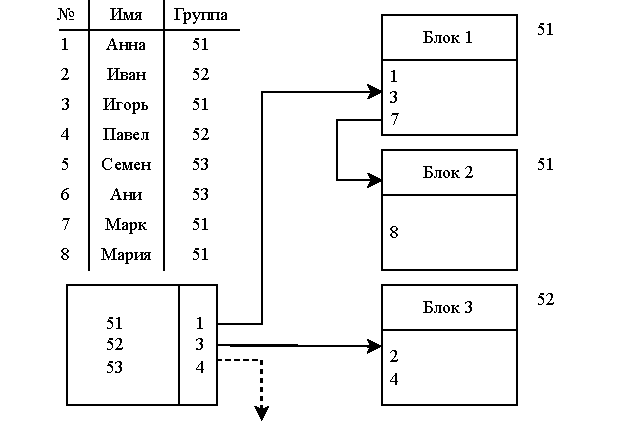
\includegraphics[scale=1.4]{img/invert.pdf}
	\caption{Пример организации инвертированных списков}
	\label{invert}
\end{figure}\pagebreak

Реляционная модель данных включает следующие компоненты~\cite{avrunev-db-models-2018}:

\begin{itemize}[label=---]
	\item структурный,
	
	\item целостный,
	
	\item манипуляционный.
\end{itemize}

В структурной части модели фиксируется, что единственной структурой данных, используемой в реляционных базах данных, является
нормализованное $n$-арное отношение.
В манипуляционной части модели выделяются два фундаментальных механизма управления реляционными базами данных: 
реляционная алгебра и реляционное исчисление.
В целостной части реляционной модели данных фиксируются два
базовых требования целостности, которые должны поддерживаться в
любой реляционной СУБД~\cite{avrunev-db-models-2018}. 

Кроме того, в состав реляционной модели данных включают теорию нормализации. 
Нормализация осуществляется для уменьшения числа возможных аномалий (нежелательные последствия при чтении, вставке, изменении или удалении данных) посредством приведения отношений к нормальной форме (НФ). 

Выделяют 1НФ, 2НФ, 3НФ, 4НФ, 5НФ, НФБК (нормальная форма Бойса-Кодда)~\cite{krenke-db-design-2005}. 
Однако отмечается, что зачастую нет необходимости в использовании нормальных форм четвертого порядка и выше~\cite{shilin-NF-2016}.  
Отношение находится в третьей нормальной форме, если оно находится во второй нормальной форме и не имеет транзитивных зависимостей \cite{krenke-db-design-2005}.

В рамках постреляционной модели выделяют распределенные файловые системы, NoSQL (Not Only SQL) СУБД, объектные, объектно-реляционные базы данных. 
Отмечается, что наилучшим решением для корпоративной информационной системы оказались многопользовательские централизованные и распределенные базы на основе строго типизированной реляционной модели с транзакционной обработкой данных. 
Однако в системах, где, например, возможно создание новых моделей данных, не требующих строго фиксированной структуры, или постоянное расширение круга пользователей, используются именно постреляционные СУБД~\cite{parfenov-postrelational-db-2016}.

\subsubsection{Архитектура организации хранения данных}

В данной классификации выделяют централизованные СУБД, которые работают с БД, которая физически хранится в одном месте (на одном компьютере). 
Это не означает, что пользователь может работать с БД только за этим же компьютером: доступ может быть удаленным, в режиме клиент–сервер. 
Кроме того, выделяются распределенные СУБД: части системы могут размещаться на двух и более компьютерах \cite{karpova-db-textbook-2009}. 

\subsection{Сущности проектируемой базы данных}

На основе выявленных требований к базе данных и хранимой информации уместно выделить следующие сущности: текст, предложение и слово. 

Более подробное разбиение текста на разделы, главы, пункты (или другие структурные единицы текста) нецелесообразно, поскольку в зависимости от жанра их наличие может варьироваться. 
Что касается дополнительной декомпозиции предложений, хранение фраз или словосочетаний также нецелесообразно, поскольку в условиях расширяемости до любого количества языков трудно предусмотреть особенности группировки слов абсолютно каждого языка. 
Кроме того, затруднено выравнивание фраз в предложениях.

Что касается разметки, уместно выделить каждый вид разметки в отдельную сущность для возможности последующего расширения. 
В базу данных будем добавлять морфологическую аннотацию и метаразметку текстов. 
Синтаксическая и семантическая разметка не будут использоваться, так как они используются в основном при специализированных исследованиях.

Кроме того, выделим такие сущности как <<язык>>, <<языковая пара>> для разграничения текстов на разных языках.

В связи с необходимостью обеспечения возможности совместного использования корпуса, необходимо также хранить минимальную информацию о пользователях: фамилию, имя, почту для обратной связи и страну, выделенную в отдельную сущность. 
Хранение страны необходимо для возможного последующего подсчета статистики по использованию корпуса.

Диаграмма <<сущность-связь>> в нотации Чена представлена на рисунке~\ref{erd}.

\begin{figure}[ht]
	\centering
	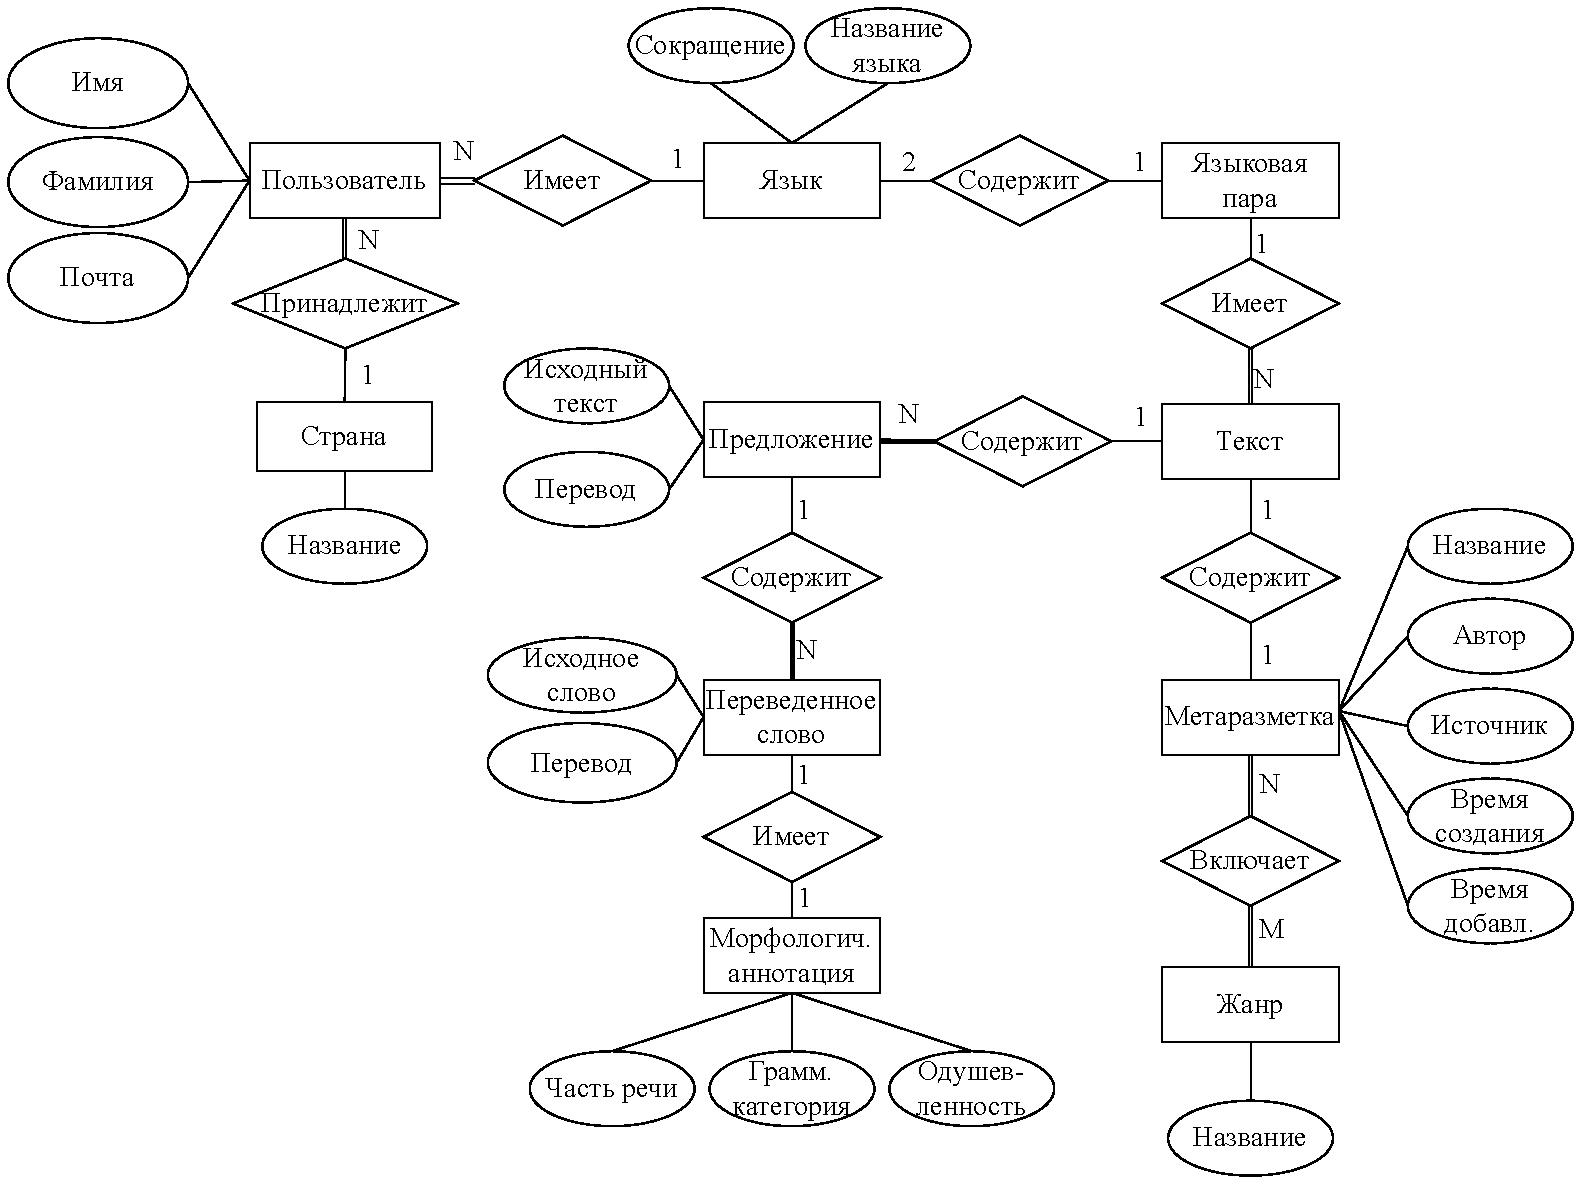
\includegraphics[width=\textwidth]{img/ERD.pdf}
	\caption{ER-диаграмма базы данных}
	\label{erd}
\end{figure}\pagebreak

\subsection{Описание пользователей проектируемого приложения к базе данных}\label{users}

Чтобы формализовать пользователей, необходимо четко сформулировать цель корпуса. 
В данном случае, это помощь в работе переводчикам и преподавателям иностранных языков. 
Таким образом, выделяются роли переводчика и преподавателя. 
Их различие состоит в отсутствии необходимости загрузки новых переведенных текстов в систему у преподавателя. Преподаватель занимается поиском контекста употребления слов, когда как переводчик может загружать новые тексты (например, из собственной практики). 
Также уместно выделить роль администратора, который будет управлять пользователями, и неавторизованного пользователя, который впоследствии станет переводчиком или преподавателем.

Диаграмма вариантов использования представлена на рисунке~\ref{use-case}.

\begin{figure}[ht]
	\centering
	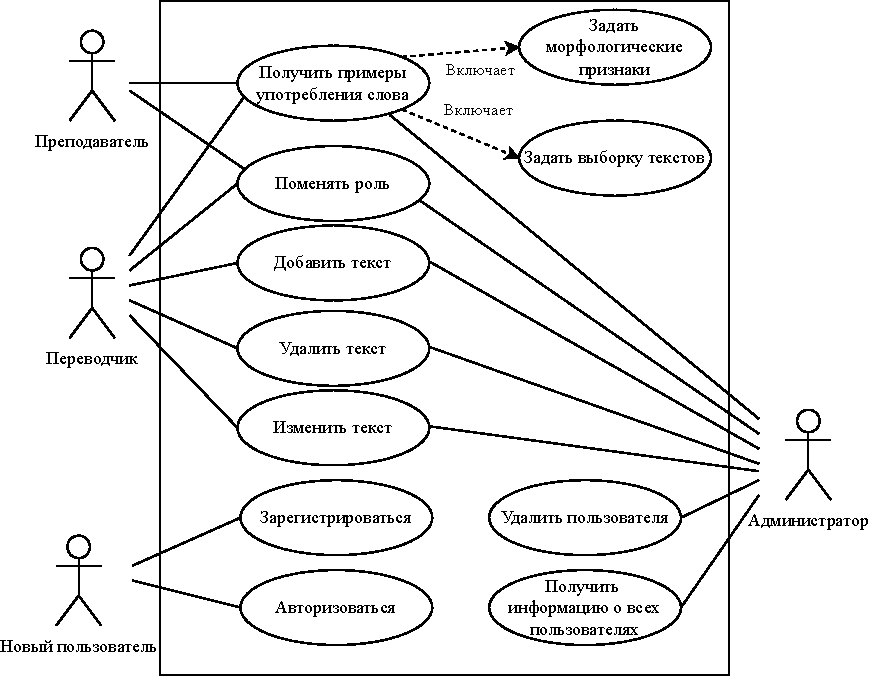
\includegraphics[width=\textwidth]{img/use-case.pdf}
	\caption{Диаграмма вариантов использования}
	\label{use-case}
\end{figure}

Для поддержания качества загружаемых текстов, администратор должен иметь возможность удалять и изменять загруженные тексты, а также удалять недобросовестных пользователей. 
Переводчик также может изменять и удалять тексты, но только самостоятельно загруженные. 
И преподаватель, и переводчик должны иметь возможность получить примеры употребления заданного слова, возможно, с указанием необходимых морфологических признаков и требуемой категории текстов.

\subsection*{Вывод}

В данном разделе была рассмотрена предметная область корпусов переведенных текстов: были даны определения ключевым понятиям области параллельных корпусов, рассмотрены варианты использования корпуса. 
Кроме того, были сформулированы требования к наполнению корпуса и его возможностям.

Из рассмотренных видов разметки для разрабатываемой базы данных выбрана морфологическая аннотация и метаразметка. 
Использование синтаксической или семантической разметки нецелесообразно, поскольку данные виды разметки используются, как правило, лишь при специализированных исследованиях.

Были также рассмотрены существующие решения и выявлен их главный недостаток -- отсутствие возможности фильтрации текстов по тематике для получения наиболее релевантных результатов. 
Кроме того, зачастую готовые решения хранят данные в устаревшем формате XML и лишь недавно начали появляться продукты, использующие современные разработки в области баз данных.

Из анализа существующих решений можно сделать вывод, что наиболее подходящим для решения поставленной задачи видом СУБД является реляционная база данных, развернутая локально (централизованная СУБД).

На основе выявленных требований к базе данных и хранимой информации выделены сущности <<текст>>, <<предложение>>, <<слово>>, <<предложение>> и другие. 
Были также разработаны и представлены на диаграмме <<сущность-связь>> связи между сущностями.

Наконец, были формализованы пользователи приложения к базе данных и их возможности, которые были представлены на диаграмме вариантов использования.

\pagebreak
